%% PHOTOELECTRIC EFFECT LOW FREQUENCY
%%%% https://tikz.net/photoelectric_effect/ %%%%
\documentclass{standalone}


%%%% https://tikz.net/photoelectric_effect/ %%%%


\IfStandalone{\def\datapath{../../../}}{\def\datapath{}}


\IfStandalone{\def\datapath{../../../}}{\def\datapath{}}

\usepackage{xcolor}
\definecolor{SciencePurple}{HTML}{663399}
\definecolor{ScienceBlue}{HTML}{214CCE}
\definecolor{ScienceGreen}{HTML}{007510}
\definecolor{ScienceYellow}{HTML}{ffbf00}
\definecolor{ScienceOrange}{HTML}{ff8c00}
\definecolor{ScienceRed}{HTML}{dc143c}
\usepackage{fontspec}
	\setmainfont{Roboto Slab}
	\setsansfont{Lato}
	\renewcommand{\familydefault}{\sfdefault}
	\setlength{\intextsep}{4pt} % Set defualt spacing around floats
	\definecolor{CommentGreen}{HTML}{228B22}
%	\captionsetup{aboveskip=5pt, belowskip=5pt} % Reduce space around captions

%% Math Env Text Settings
\usepackage{mathtools}
\usepackage{unicode-math}
	\setmathfont{XITS Math}
\usepackage{amsmath}
\usepackage{bm}
%	\everymath=\expandafter{\the\everymath\displaystyle}


%% https://tex.stackexchange.com/questions/8434/how-to-scale-math-font-only#8448
\DeclareMathSizes{11pt}{12pt}{7pt}{7pt}
\DeclareMathSizes{14pt}{15pt}{9pt}{9pt}

%% https://tex.stackexchange.com/questions/122574/globally-changing-math-line-spacing
\setlength{\jot}{7pt}

%% https://www.overleaf.com/learn/latex/Spacing_in_math_mode
%% https://tex.stackexchange.com/questions/41913/how-to-get-less-spacing-in-math-mode
%% https://mirror.kumi.systems/ctan/obsolete/info/math/voss/mathmode/Mathmode.pdf
\thinmuskip=5mu % (by default it is equal to 3 mu)
\medmuskip=5mu  % (by default it is equal to 4 mu)
\thickmuskip=7mu  % (by default it is equal to 5 mu)


\usepackage{tikz}
\usepackage{siunitx}
\usepackage{pgfplots}

\usepackage{physics}
\usepackage{etoolbox} %ifthen
\usepackage[outline]{contour} % glow around text


%%%%%%%%%% PGFPLOTS & PGFPLOTS SETTINGS %%%%%%%%%%
\pgfplotsset{compat=newest,
	width=6cm,
	height=3cm,
	scale only axis=true,
	max space between ticks=25pt,
	try min ticks=5,
	every axis/.style={
		axis y line=left,
		axis x line=bottom,
		axis line style={thick,->,>=latex, shorten >=-.4cm}
	},
	every axis plot/.append style={thick},
	tick style={black, thick}
}
\tikzset{
	semithick/.style={line width=0.8pt},
}

\usepgfplotslibrary{groupplots}
\usepgfplotslibrary{dateplot}

% Circuits
\usepackage{circuitikz}
%% Specifications
\ctikzset{bipoles/thickness=1.2}

% Styles
\tikzset{>=latex}

% Tikz Library
\usetikzlibrary{angles,quotes}

% Define Color
\tikzstyle{bigphoton}=[-{Latex[length=8,width=6]},red!95!black!50,opacity=0.85,very thin,decorate,decoration={snake,amplitude=2.8,segment length=8,post length=8}]



%%%% https://tikz.net/function_average/ %%%%
\usepackage{physics}
\usepackage[outline]{contour} % glow around text
\contourlength{1.0pt}

\tikzset{>=latex} % for LaTeX arrow head
\colorlet{myred_}{red!85!black}
\colorlet{myblue_}{blue!80!black}
\colorlet{mydarkred_}{myred_!80!black}
\colorlet{mydarkblue_}{myblue_!60!black}
\tikzstyle{xline}=[myblue_,thick]
\def\tick#1#2{\draw[thick] (#1) ++ (#2:0.09) --++ (#2-180:0.18)}
\tikzstyle{myarr_}=[myblue_!50,-{Latex[length=3,width=2]}]
\def\N{100}


\begin{document}
	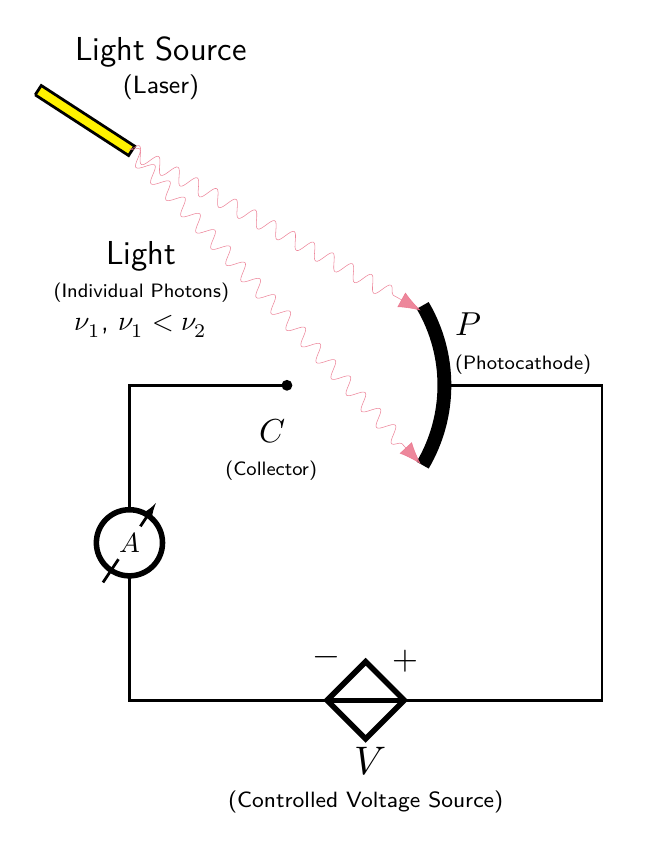
\begin{tikzpicture}[scale=1, line width=1]
		% Grid
		%				\draw[help lines] (0,0) grid (11,11);
		
		% Circuits		
		\draw (4,6) -- (2,6) to[rmeterwa, t=$A$] ++(0,-4) -- (2,2) to[controlled voltage source, l_={
			\begin{tabular}{c}
				\Large $V$ \\
				\footnotesize (Controlled Voltage Source)
		\end{tabular}}] ++(6,0) -- (8,6) -- (6,6);
		\filldraw (4,6) circle [radius=0.05];
		
		% Dashed Arrows
		\draw[color=ScienceGreen,opacity=0,dashed,<-] (4,6) -- +(1.7,1)coordinate(A);
		\draw[color=ScienceGreen,opacity=0,dashed,<-] (4,6)coordinate(B) -- +(1.7,-1)coordinate(C);
		
		% Arc		
		\pic [draw, angle radius = 2cm, line width = 5] {angle=C--B--A};
		
		% Photocell
		\draw[color=black, line width=5, opacity=0] (5,6) circle [radius=1.8];
		
		% Laser
		\draw[fill=yellow, line width=1, rotate=12] (2.8,9.31) -- ++(1,-1) -- ++(0.1,0.1) -- ++(-1,1) -- +(-0.1,-0.1);
		%% Rays
		\draw[bigphoton,ScienceRed!60] (2,9) -- (5.7,5);
		\draw[bigphoton,ScienceRed!60] (2,9) -- (5.7,6.95);
		
		
		% Nodes
		\node at (5.5,2.5) {\large $+$};
		\node at (4.5,2.5) {\large $-$};
		\node at (3.8,5.15) {
			\begin{tabular}{c}
				\large $C$ \\
				\scriptsize (Collector)
		\end{tabular}};
		\node at (7,6.5) {
			\begin{tabular}{l}
				\large $P$ \\
				\scriptsize (Photocathode)
		\end{tabular}};
		\node at (2.4,10) {
			\begin{tabular}{c}
				\large Light Source \\
				\small (Laser)
		\end{tabular}};
		\node at (2.15,7.2) {
			\begin{tabular}{c}
				\large Light \\
				\scriptsize (Individual Photons) \\
				\normalsize $ \nu_1 $, $\nu_1 < \nu_2$
		\end{tabular}};
	\end{tikzpicture}
\end{document}